\documentclass{beamer}
\usetheme[faculty=econ]{fibeamer}

\usepackage[utf8]{inputenc}
\usepackage[francais]{babel}
\usepackage[T1]{fontenc}
\usepackage{xcolor}

\lstset{
	language=Java,                
	basicstyle=\scriptsize,
	escapeinside={*@}{*@},
	frame=single,
	xleftmargin=2mm,
	xrightmargin=2mm,
	keepspaces=true,
	tabsize=2
}
\newcounter{ctr1}
\title[]{\Large{Développement d'applications modulaires en Java}}
\author[C. Tibermacine]{\large{Chouki~Tibermacine}\\
	\small{Chouki.Tibermacine@umontpellier.fr}}
%\institute{Polytech Montpellier}
\date{\tiny{}}

\begin{document}

\begin{frame}
\titlepage
\begin{flushright}

\includegraphics[width=3.5cm]{figs/polytech.png}
\end{flushright}
\end{frame}

\begin{frame}
	\frametitle{Plan de l'ECUE}
	\begin{enumerate}
		\item (Rappels sur le) Développement d'applications Web avec Java
		\item Modulariser les applications Java avec Spring
		\item Bien structurer une application Web avec Spring MVC
		\item Auto-configurer une application Web avec Spring Boot
		\item Sécuriser une application Web avec Spring Security
		\item Gérer des données massives avec Apache Kafka et Spring
		\item Tester une application Web Spring
		\item Écrire des applications Web (API) réactives avec Spring WebFlux
	\end{enumerate}
\end{frame}

\begin{frame}
	\frametitle{Plan de l'ECUE}
	\begin{enumerate}
		{\color{gray}{
		\item (Rappels sur le) Développement d'applications Web avec Java}}
				\item Modulariser les applications Java avec Spring
		{\color{gray}{
				\item Bien structurer une application Web avec Spring MVC
				\item Auto-configurer une application Web avec Spring Boot
				\item Sécuriser une application Web avec Spring Security
				\item Gérer des données massives avec Apache Kafka et Spring		
				\item Tester une application Web Spring
				\item Écrire des applications Web (API) réactives avec Spring WebFlux}}
	\end{enumerate}
\end{frame}

\begin{frame}
  \frametitle{Livres de référence}
  \begin{tikzpicture}[overlay,remember picture]
    \node[anchor=center,xshift=-120pt,yshift=-20pt]
    at (current page.center) {
      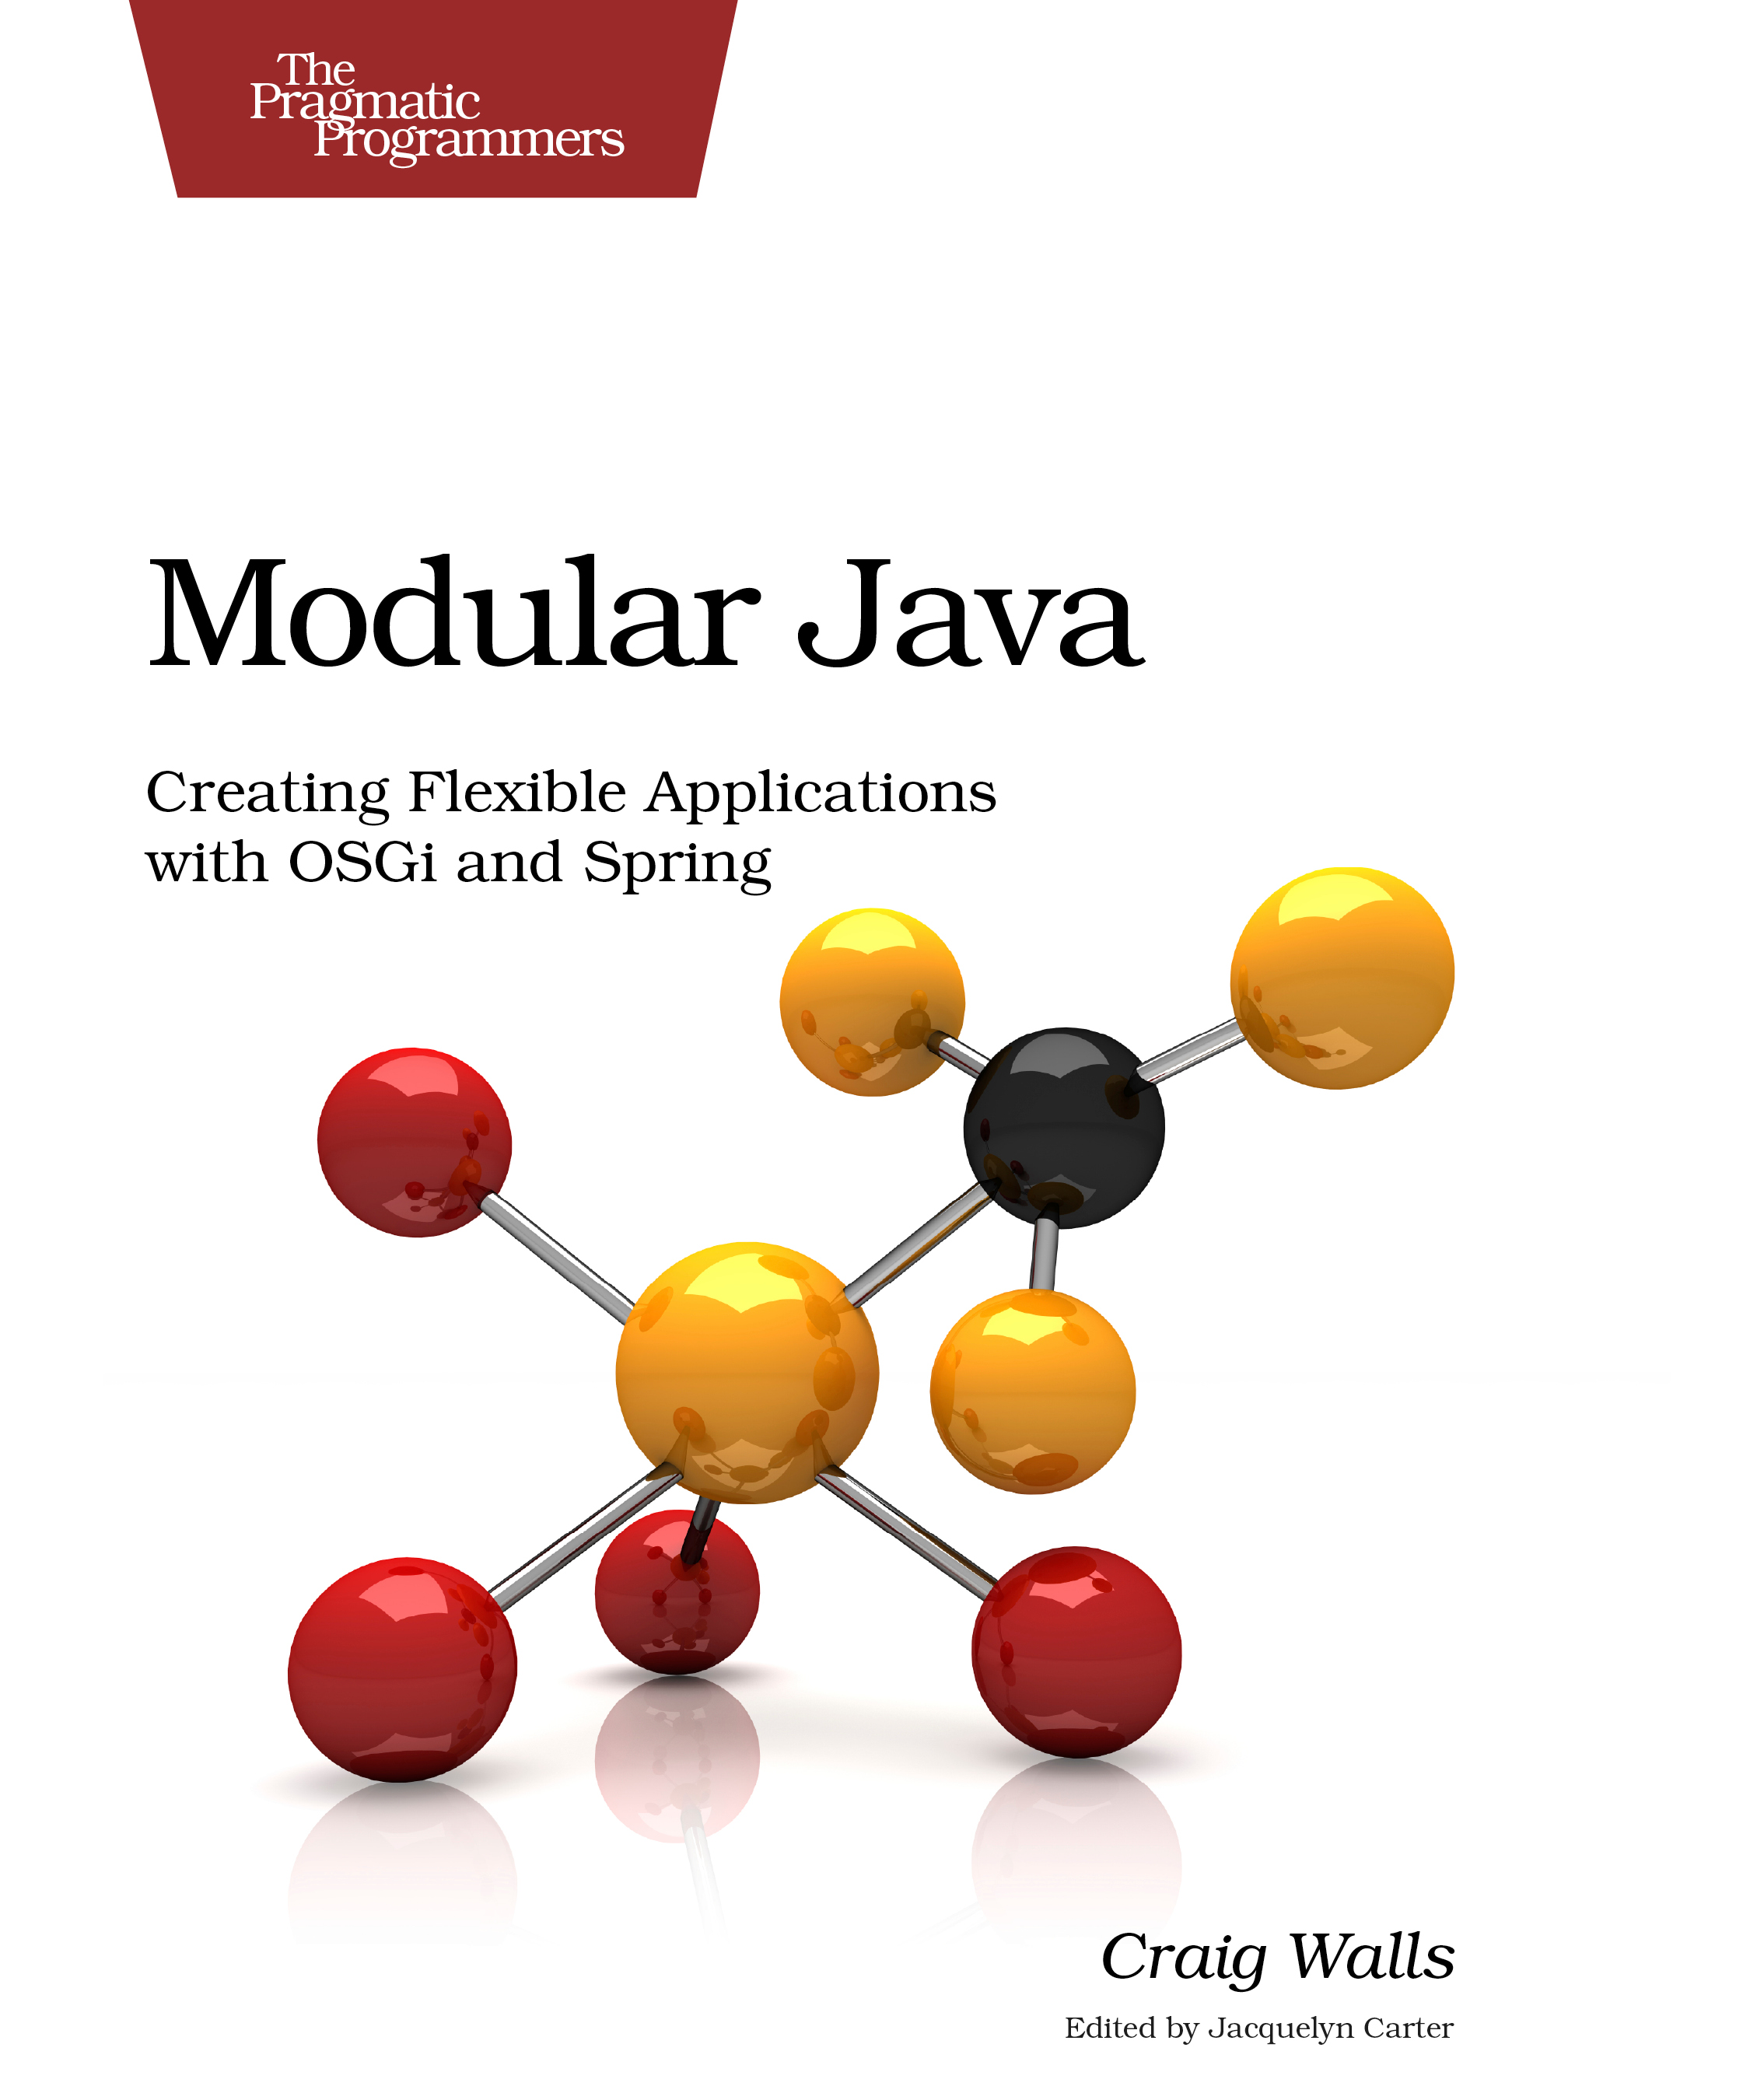
\includegraphics[width=4cm]{img/book1.jpg}
    };
  \end{tikzpicture}
  \begin{tikzpicture}[overlay,remember picture]
    \node[anchor=center,xshift=0pt,yshift=-20pt]
    at (current page.center) {
      
\includegraphics[width=4cm]{img/book2.png}
    };
  \end{tikzpicture}
  \begin{tikzpicture}[overlay,remember picture]
    \node[anchor=center,xshift=120pt,yshift=-20pt]
    at (current page.center) {
      
\includegraphics[width=4cm]{img/book3.png}
    };
  \end{tikzpicture}    
\end{frame}

\AtBeginSection[]{% Print an outline at the beginning of sections
  \begin{frame}<beamer>
    \frametitle{Plan du cours}
    % \frametitle{Outline}
    \tableofcontents[currentsection]
    % \tableofcontents
  \end{frame}}

\AtBeginSubsection[]{% Print an outline at the beginning of sections
  \begin{frame}<beamer>
    \frametitle{Plan du cours}
    % \frametitle{Outline}
    \tableofcontents[currentsubsection]
    % \tableofcontents
  \end{frame}}
\section{Introduction à la programmation modulaire en Java}

\begin{frame}
  \frametitle{Qu'est-ce qu'un module ?}  
  \begin{itemize}
  \item Module = unité de code indépendante dans un système logiciel
  \item Deux caractéristiques fondamentales :
    \begin{itemize}
    \item Forte cohésion : le module se focalise sur une tâche unique
    \item Couplage minimal : le module a de faibles dépendances avec les
      autres modules
    \end{itemize}
  \item La modularité existe depuis longtemps (le langage Modula dans
    les années 70, un des ancêtres de Java)    
  \end{itemize}
\end{frame}

\begin{frame}
  \frametitle{Description d'un module}  
  \begin{itemize}
  \item A l'origine, un module est décrit par :
    \begin{enumerate}
    \item Une spécification du module : signatures des fonctions publiques
	fournies par le module\\
        $\sim$ une interface Java
      \item Une implémentation du module : implémentation des
        fonctions fournies\\
        $\sim$ une classe Java qui implémente l'interface
      \end{enumerate}
    \item La plupart des langages de programmation par objets
      fournissent les moyens pour organiser son code ainsi
  \end{itemize}
\end{frame}

\begin{frame}
  \frametitle{Intérêt de la modularité}  
  \begin{itemize}
  \item  \textbf{Maintenabilité :}
    \begin{itemize}
    \item Module = unité facilement compréhensible indépendamment des
      autres modules (comparativement à un système complet)
      \item Module =
      unité pouvant être changée (son implémentation) sans grand
      impact sur les autres modules (qui sont liés à l'interface)
    \end{itemize}
    \item \textbf{Réutilisabilité :}
    \begin{itemize}      
    \item Module = unité facilement réutilisable dans d'autres
      contextes (faisant partie d'autres applications)
    \end{itemize}
  \item \textbf{Testabilité :}
    \begin{itemize}      
    \item Module = unité sur laquelle les tests unitaires peuvent être
      facilement réalisés
    \end{itemize}
  \end{itemize}
\end{frame}

\begin{frame}
  \frametitle{Du module au composant}
  \begin{tikzpicture}[overlay,remember picture]
    \node[anchor=center,xshift=0pt,yshift=0pt]
    at (current page.center) {
      
\includegraphics[width=1cm]{img/fleche.jpg}
    };
  \end{tikzpicture}
      \begin{center}  
%  \begin{itemize}
 De la « Séparation Spécification-Implémentation »\\
\vspace{3cm}    
 À la « Séparation Logique -Architecture »\\
\vspace{1cm}
Composant = Module++

  \end{center}
\end{frame}

\begin{frame}
  \frametitle{Rappel de ce qu'est un composant}  
  \begin{itemize}
  \item  Un composant est une unité logicielle qui :
    \begin{itemize}
    \item décrit de façon explicite ses :
    \begin{enumerate}
    \item fonctionnalités fournies : signatures des opérations qu'il offre
(comme dans les modules)
\item fonctionnalités requises : signatures des opérations dont il
	a besoin pour implémenter les fonctionnalités fournies
\item son architecture interne : liste des instances de ses
	composants internes et leurs interconnexions
    \end{enumerate}
\item est sujet à une instanciation et à une connexion avec d'autres
	composants (qui ont besoin de ses opérations / qui répondent
	à ses besoins -fournissent ses opérations requises-)
  \end{itemize}        
  \end{itemize}
\end{frame}

\begin{frame}
  \frametitle{Modularité dans les composants logiciels}  
  \begin{itemize}
  \item  Interfaces requises explicites :
  \begin{itemize}
  \item Un composant ne dépend pas directement d'un autre composant
  \item Il requiert un certain nombre d'opérations (spécifiées dans
    une ou plusieurs interface(s) : type abstrait) que peut fournir
    (implémenter) un autre composant
  \end{itemize}
\item Dépendances entre composants mises en place par un architecte :
  \begin{itemize}
  \item Un rôle différent de celui qui développe les composants (qui
    sont à connecter, et destinés pour la réutilisation) : développeur
    par la réutilisation
  \end{itemize}
\end{itemize}
\end{frame}

\begin{frame}
  \frametitle{Modularité dans Java : un exemple}
  \begin{tikzpicture}[overlay,remember picture]
    \node[anchor=center,xshift=0pt,yshift=-40pt]
    at (current page.center) {
      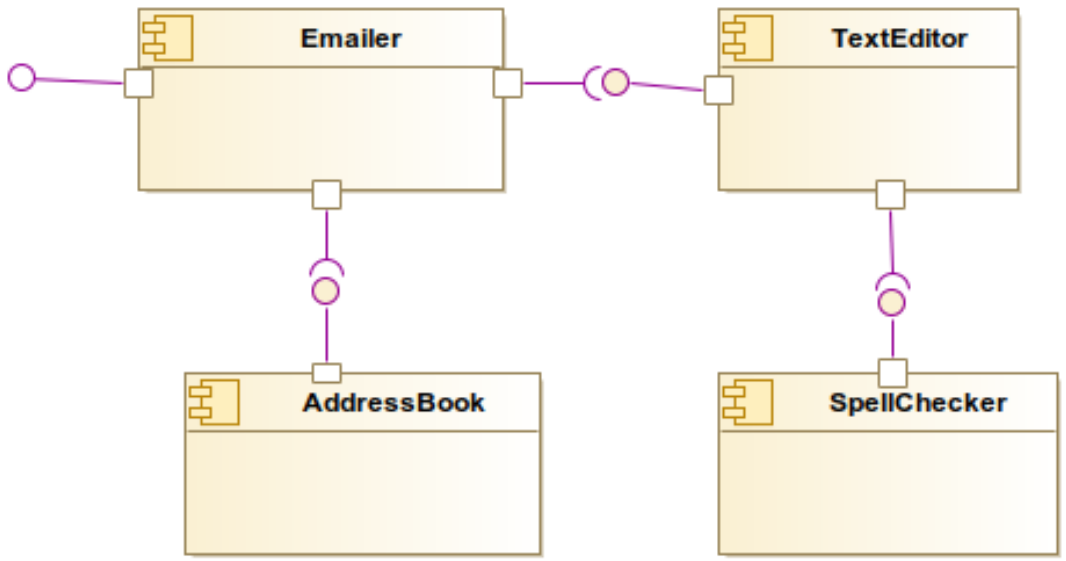
\includegraphics[width=9cm]{img/example_app.png}
    };
  \end{tikzpicture}  
  \begin{itemize}
  \item Architecture simplifiée d'un exemple jouet :
    \vspace{5cm}
  \end{itemize}
\end{frame}

\begin{frame}
  \frametitle{Composant Emailer en « UML »}
  \begin{tikzpicture}[overlay,remember picture]
    \node[anchor=center,xshift=0pt,yshift=-40pt]
    at (current page.center) {
      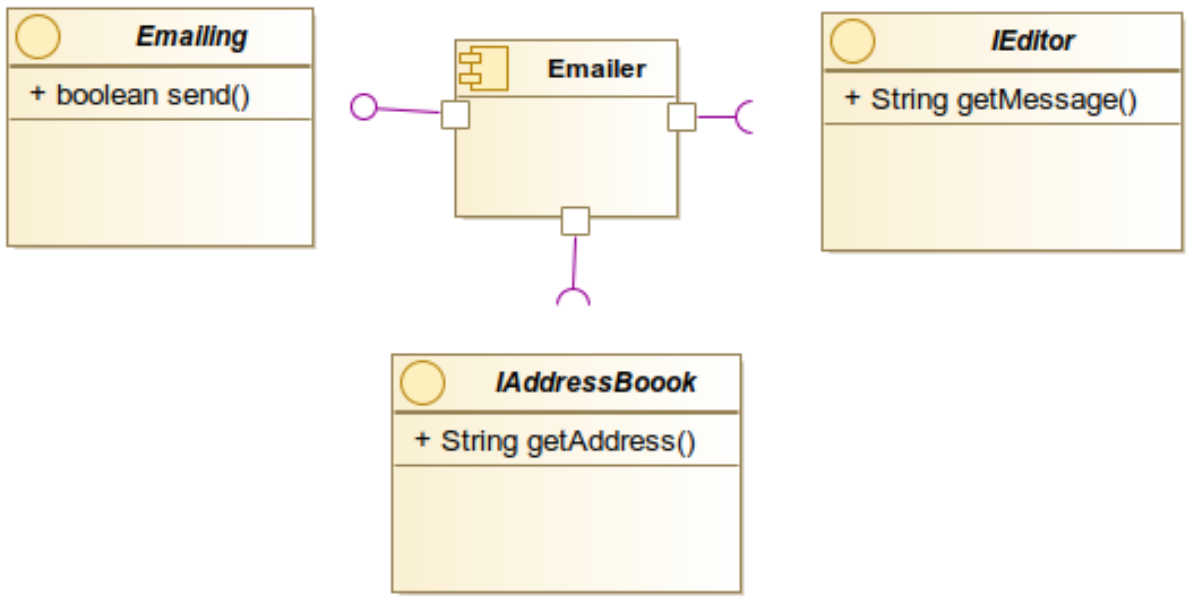
\includegraphics[width=10cm]{img/comp_emailer.png}
    };
  \end{tikzpicture}  
  \begin{itemize}
  \item Interface fournie et interfaces requises :
    \vspace{5cm}
  \end{itemize}
\end{frame}

\begin{frame}[fragile]
  \frametitle{Composant Emailer en Java}
  \begin{itemize}
  \item Une simple classe :
    \end{itemize}
\begin{lstlisting}[language=Java]
public class Emailer implements Emailing {
  public IEditor editor;
  public IAddressBook addressBook;
  
  // Constructeurs ...

  public boolean send() {
    String msg = editor.getMessage();
    String address = addressBook.getAddress();
    return sendMessage(msg,address); // Methode locale
  }
}
\end{lstlisting}
\end{frame}

\begin{frame}[fragile]
  \frametitle{Composant Emailer en Java}
  \begin{tikzpicture}[overlay,remember picture]
    \node[anchor=east,xshift=-25pt,yshift=70pt]
    at (current page.east) {
      
\includegraphics[width=4cm]{img/prov_intf.png}
    };
  \end{tikzpicture}      

\begin{lstlisting}[language=Java]
public class Emailer implements *@\normalsize{\textbf{Emailing}}*@ {
  public IEditor editor;
  public IAddressBook addressBook;
  
  // Constructeurs ...

  public boolean send() {
    String msg = editor.getMessage();
    String address = addressBook.getAddress();
    return sendMessage(msg,address); // Methode locale
  }
}
\end{lstlisting}
\end{frame}

\begin{frame}[fragile]
  \frametitle{Composant Emailer en Java}
  \begin{tikzpicture}[overlay,remember picture]
    \node[anchor=east,xshift=-25pt,yshift=70pt]
    at (current page.east) {
      
\includegraphics[width=4cm]{img/prov_intf.png}
    };
  \end{tikzpicture}
  \begin{tikzpicture}[overlay,remember picture]
    \node[anchor=east,xshift=-35pt,yshift=30pt]
    at (current page.east) {
      
\includegraphics[width=3cm]{img/req_intf.png}
    };
  \end{tikzpicture}  

\begin{lstlisting}[language=Java]
public class Emailer implements *@\normalsize{\textbf{Emailing}}*@ {
  public *@\textbf{IEditor}*@ editor;
  public *@\textbf{IAddressBook}*@ addressBook;
  
  // Constructeurs ...

  public boolean send() {
    String msg = editor.getMessage();
    String address = addressBook.getAddress();
    return sendMessage(msg,address); // Methode locale
  }
}
\end{lstlisting}
\end{frame}

\begin{frame}
  \frametitle{Composant TextEditor en « UML »}
  \begin{tikzpicture}[overlay,remember picture]
    \node[anchor=center,xshift=0pt,yshift=-40pt]
    at (current page.center) {
      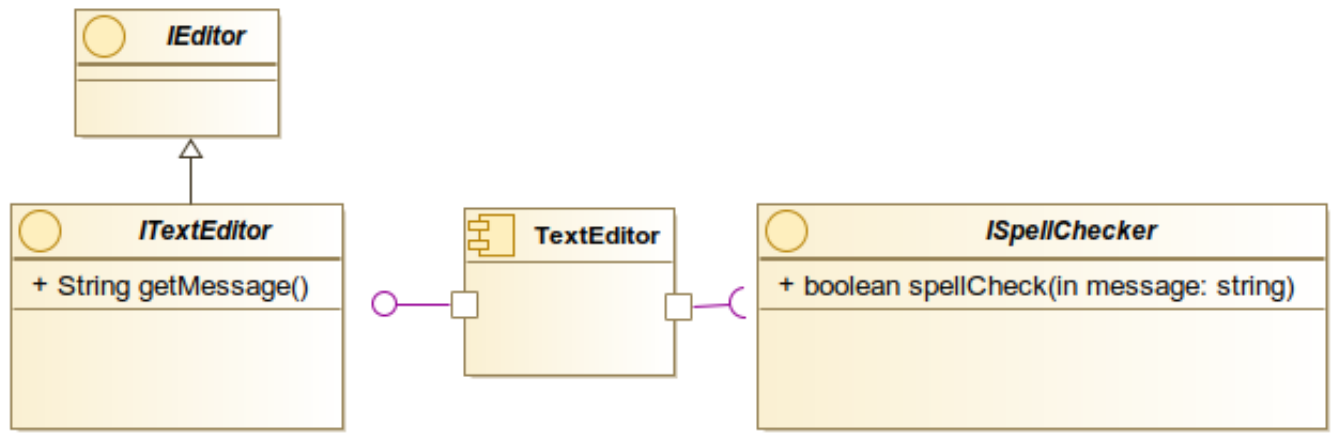
\includegraphics[width=10cm]{img/comp_texteditor.png}
    };
  \end{tikzpicture}  
  \begin{itemize}
  \item Interface fournie et interfaces requises :
    \vspace{5cm}
  \end{itemize}
\end{frame}

\begin{frame}[fragile]
  \frametitle{Composant TextEditor en Java}
  \begin{itemize}
  \item Une simple classe :
  \end{itemize}
\begin{lstlisting}[language=Java]
public class TextEditor implements ITextEditor {
  public ISpellChecker checker;

  // Constructeurs ...
  
  public String getMessage() {
    ... {
      String msg = getUserInput();// Methode locale
      boolean isCorrect = checker.spellCheck(msg);
      if(isCorrect) return msg;
    }
  }
}
\end{lstlisting}
\end{frame}

\begin{frame}[fragile]
  \frametitle{Composant TextEditor en Java}
  \begin{itemize}
  \item Une simple classe :
  \end{itemize}
\begin{lstlisting}[language=Java]
public class TextEditor implements *@\textbf{ITextEditor}*@ {
  public *@\textbf{ISpellChecker}*@ checker;

  // Constructeurs ...
  
  public String getMessage() {
    ... {
      String msg = getUserInput();// Methode locale
      boolean isCorrect = *@\textbf{checker}*@.spellCheck(msg);
      if(isCorrect) return msg;
    }
  }
}
\end{lstlisting}
\end{frame}

\begin{frame}
  \frametitle{Décrire l'architecture et lancer l'application}  
  \begin{itemize}
  \item Définir une classe avec un main dans laquelle on instancie les
    différentes classes qui représentent les composants

  \item Les dépendances entre ces composants sont résolues de deux
    façons :
  \begin{itemize}
  \item En initialisant les attributs (interfaces requises) avec des
    références aux instances créés -- solution 1
  \item En passant ces références sous la forme d'arguments aux
    constructeurs des différentes classes au moment de l'instanciation
    -- solution 2
  \end{itemize}
\end{itemize}
\end{frame}

\begin{frame}[fragile]
  \frametitle{Décrire l'architecture -- Solution 1} 
  \begin{itemize}
  \item Classe de description d'archi. et de lancement de
    l'application :
  \end{itemize}
  \begin{lstlisting}[language=Java]    
public class MainApplication {
  private static Emailing emailer;
  private static void configureApplication() {
    emailer = new Emailer();
    ITextEditor editor = new TextEditor();
    editor.setChecker(new SpellChecker());
    emailer.setEditor(editor);
    emailer.setAddressBook(new AddressBook());
  }
  public static void main(String... args) {
    configureApplication();
    emailer.send();
  }
}
  \end{lstlisting}  
\end{frame}

\begin{frame}[fragile]
  \frametitle{Décrire l'architecture -- Solution 2} 
  \begin{itemize}
  \item Classe de description d'archi. et de lancement de
    l'application :
  \end{itemize}
  \begin{lstlisting}[language=Java]
public class MainApplication {
  private static Emailing emailer;
  private static void configureApplication() {
    ISpellChecker checker = new SpellChecker();
    IEditor editor = new TextEditor(checker);
    IAddressBook book = new AddressBook();
    emailer = new Emailer(editor,book);
  }
  public static void main(String... args) {
    configureApplication();
    System.out.println(emailer.send());
  }
}
  \end{lstlisting}  
\end{frame}

\begin{frame}[fragile]
  \frametitle{Constructeur de la classe Emailer} 
  \begin{lstlisting}[language=Java]
public class Emailer implements Emailing {
  public IEditor editor;
  public IAddressBook addressBook;
  public Emailer(IEditor e, IAddressBook a) {
    this.editor = e;
    this.addressBook = a;
  }
  public boolean send() {
    // ...
  }
}
  \end{lstlisting}  
\end{frame}

\begin{frame}[fragile]
  \frametitle{Avoir des dépendances noyées dans le code} 
  \begin{lstlisting}[language=Java]
public class TextEditor implements ITextEditor {
      
  public ISpellChecker checker;

  public TextEditor() {
    checker = new EnglishSpellChecker();
  }

  // ...
}
  \end{lstlisting}  
\end{frame}
\begin{frame}[fragile]
  \frametitle{Avoir des dépendances noyées dans le code}
  \begin{tikzpicture}[overlay,remember picture]
    \node[anchor=center,xshift=0pt,yshift=-50pt]
    at (current page.center) {
      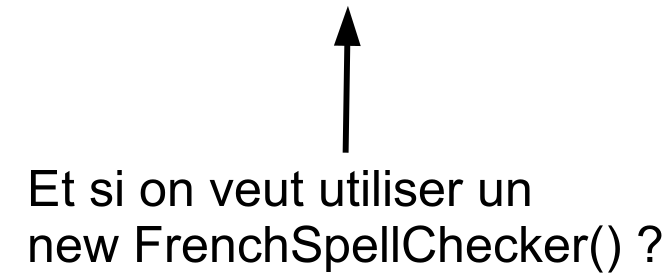
\includegraphics[width=4cm]{img/deps_noyees.png}
    };
  \end{tikzpicture}    
  \begin{lstlisting}[language=Java]
public class TextEditor implements ITextEditor {
      
  public ISpellChecker checker;

  public TextEditor() {
    checker = new EnglishSpellChecker();
  }

  // ...
}
  \end{lstlisting}  
\end{frame}

\begin{frame}
  \frametitle{Avantages de la solution : constructeur avec paramètres}  
  \begin{itemize}
  \item Dépendances entre composants peuvent être définies depuis
    l'extérieur par l'architecte de l'application et non par le
    développeur du composant Emailer
\item Séparation des préoccupations :
  \begin{itemize}
  \item Code représentant la logique de l'application séparé du
    code décrivant l'architecture de celle-ci

  \item C'est la classe MainApplication qui s'occupe de la description
    d'architecture
  \end{itemize}
\end{itemize}
\end{frame}

\begin{frame}[fragile]
  \frametitle{Avantages de la solution : attributs typés par des
    interfaces requises}
  \begin{itemize}
  \item Possibilité de connecter n'importe quel composant, qui implémente
    l'interface requise (ou interface dérivée)
  \begin{itemize}   
  \item Le composant requiert une spécification abstraite
  \item Il ne dépend pas d'une implémentation particulière
  \end{itemize}
\item Exemple :
  \begin{lstlisting}[language=Java]
public class FrenchSpellChecker
             implements ISpellChecker {
  public String spellCheck() { /* ... */ }
}
\end{lstlisting}
Le composant TextEditor peut être connecté à une instance
de FrenchSpellChecker :
  \begin{lstlisting}[language=Java]
IEditor editor = new TextEditor(new FrenchSpellChecker());
\end{lstlisting}
  \end{itemize}
\end{frame}

\begin{frame}
  \frametitle{Peut mieux faire !!!}
  \begin{itemize}
  \item Au lieu de gérer la création de ces instances et leur
    connexion, demander ça à des objets tiers
  \item Ces objets peuvent être distants. Ils centralisent des pools
    d'objets (qui peuvent être uniques), qui peuvent avoir accès à
    certaines ressources « précieuses »
  \item Le programmeur est déchargé de cela. Il doit s'occuper de la
    logique métier de son application
  \end{itemize}
\end{frame}


\section{Quelques patrons de conception pour la modularité}

\begin{frame}
  \frametitle{Patron « Factory » ou « Abstract Factory »}  
  \begin{itemize}
  \item Le patron « Factory » (ou « Abstract Factory ») préconise la
    définition d'une classe qui crée des instances et gère leurs
    dépendances
  \item Pour notre exemple, on peut écrire une classe EmailerFactory
    avec une méthode qui ressemble à la méthode configureApplication()
  \end{itemize}
\end{frame}

\begin{frame}[fragile]
  \frametitle{Exemple avec ce patron}  
\begin{lstlisting}[language=Java]
public class EmailerFactory {
  public Emailing newFrenchEmailer() {
    ISpellChecker checker = new FrenchSpellChecker();
    IEditor editor = new TextEditor(checker);
    IAddressBook book = new AddressBook();
    Emailer emailer = new Emailer(editor,book);
    return emailer;
  }
  public Emailing newGermanEmailer() {
    ISpellChecker checker = new GermanSpellChecker();
    // ...
  }
}
\end{lstlisting}
\end{frame}

\begin{frame}[fragile]
  \frametitle{Avantages de ce patron}  
  \begin{itemize}
  \item Un composant client (notre MainApplication, dans l'exemple)
est déchargé de ce travail d'instanciation et de gestion
des dépendances entre objets
\item Un composant client n'a besoin de connaître que le composant
EmailerFactory (et non les autres composants)
\item Encore de la séparation des préoccupations :-)
    \begin{itemize}
  \item
Code de création d'instances et de gestion de leurs dépendances
séparé du code d'utilisation du composant Emailer :
\begin{lstlisting}[language=Java]
  new EmailerFactory().newFrenchEmailer() ...
\end{lstlisting}
ou souvent (méthode factory statique)
\begin{lstlisting}[language=Java]
  EmailerFactory.newFrenchEmailer() ...
\end{lstlisting}

  \end{itemize}
\end{itemize}
\end{frame}

\begin{frame}[fragile]
  \frametitle{Défauts de ce patron}  
  \begin{itemize}
  \item Il faudra créer autant de méthodes que de variations, dans les
    composants et leurs dépendances, qu'on souhaite obtenir avec ce «
    factory »
  \item Il faudra définir autant de méthodes new...Emailer() que de
    langues qu'on souhaite avoir pour le spell checker
  \item Et si on voudrait changer AddressBook par PhoneAndAddressBook
    \begin{itemize}
    \item Il faudra changer chacune de ces méthodes (+ combinaisons)
    \end{itemize}
  \end{itemize}
\end{frame}

\begin{frame}[fragile]
  \frametitle{Patron « Service Locator »}  
  \begin{itemize}
  \item Le patron « Service Locator » est une sorte de « factory »
  \item Il s'agit d'un objet tiers utilisé pour obtenir une instance
    ayant toutes ses dépendances résolues
  \item Ça peut être un objet qui s'exécute sur la même machine
    virtuelle que les autres composants de l'application qu'on
    construit, comme ça peut être un objet distant
  \item JNDI est un bon exemple de « Service Locator » utilisé dans
    les composants EJB, Web Java, ..
  \end{itemize}
\end{frame}

\begin{frame}[fragile]
  \frametitle{Exemple avec ce patron}  
  \begin{itemize}
  \item Utilisation de ce patron :
\begin{lstlisting}[language=Java]
Emailing emailer=(Emailing) new ServiceLocator()
                  .get("emailer");
\end{lstlisting}    

\item Utilisation de clés pour obtenir une référence vers un composant
  \begin{itemize}
  \item Le mot "emailer" dans notre exemple
  \end{itemize}
\item Les mêmes problèmes que nous avons avec le « Factory » se posent
  avec ce patron
\item De plus, les clés utilisées sont opaques et peuvent être
  ambigües
  \begin{itemize}
  \item Possibles erreurs à l'exécution (si la clé n'est pas correcte)
  \end{itemize}
\end{itemize}
\end{frame}

\section{Injection de dépendances avec Spring}

\subsection{Généralités sur la DI et introduction à Spring}
\begin{frame}
  \frametitle{Injection de dépendances (DI)}
  \begin{itemize}
  \item Une entité externe à l'application :
    \begin{itemize}
    \item crée les instances nécessaires
    \item les lie ensemble
    \end{itemize}
  \item De cette façon, les développeurs d'une application sont
    déchargés de cette tâche et peuvent se focaliser uniquement sur la
    programmation de la logique métier
  \end{itemize}
\end{frame}

\begin{frame}[fragile]
  \frametitle{Exemple d'injection manuelle de dépendances}
  \begin{itemize}
  \item Le constructeur de la classe Emailer (vu précédemment) :
\begin{lstlisting}[language=Java]
public Emailer(IEditor e, IAddressBook a) {
  this.editor = e;
  this.addressBook = a;
}
\end{lstlisting}        
  \item Dans une autre classe, on écrit :
\begin{lstlisting}[language=Java]
new Emailer(new TextEditor(),new AddressBook());
\end{lstlisting}          
  \item Ici, on a une injection manuelle des dépendances dans une
    instance de la classe Emailer à travers son constructeur
  \end{itemize}
\end{frame}

\begin{frame}[fragile]
  \frametitle{Frameworks d'injection automatique de dépendances}
  \begin{itemize}
  \item L'injection de dépendances peut être réalisée de façon
    automatique
  \item Il existe des frameworks Java proposant des solutions
    d'injection automatique de dépendances
  \item Quelques frameworks gratuits :
    \begin{itemize}
    \item Spring : AOP, Web MVC, ... (celui qui a popularisé la DI)
    \item Guice de Google (le plus simple)
    \item PicoContainer (l'un des premiers frameworks)
    \item Quelques projets chez Apache : Avalon et HiveMind
    \item Chez Oracle : DI dans JEE (inspirée de Spring et Guice)
    \end{itemize}
  \end{itemize}
\end{frame}

\begin{frame}[fragile]
  \frametitle{Un peu d'histoire sur Spring}
  \begin{itemize}
  \item Décembre 1996 : JavaBeans - modèle de composants Java
    \begin{itemize}
    \item se limitant principalement aux interfaces graphiques
    \end{itemize}        
  \item Mars 1998 : EJB - modèle de composants plus riche
    (transactions, persistance, ...)
    \begin{itemize}
    \item répondant aux besoins réels des applications d'entreprise
      (mais rendant le code assez complexe et verbeux)
    \end{itemize}      
  \item Juin 2003 : Spring - une simplification du développement des
    applications d'entreprise (DI, AOP, ...)
    \begin{itemize}
    \item développement de la logique métier des applications avec des
      POJOs (Plain-Old Java Objects)
    \item mise en place des autres aspects en utilisant un modèle de
      programmation déclarative
    \end{itemize}
  \end{itemize}
\end{frame}

\subsection{Définition de composants Spring}

\begin{frame}[fragile]
  \frametitle{Mettre en place l'environnement Spring}  
  \begin{itemize}
  \item Configuration Spring (fichier XML) :
    
    \begin{lstlisting}[language=XML,basicstyle=\scriptsize]
<?xml version="1.0" encoding="UTF-8" ?>
<beans
  xmlns="http://www.springframework.org/schema/beans"
  xmlns:xsi="http://www.w3.org/2001/XMLSchema-instance"
  xsi:schemaLocation="http://www.springframework.org/schema/beans
  http://www.springframework.org/schema/beans/spring-beans.xsd">
  <!-- Declarations de composants (beans) ici -->
  </beans>
  \end{lstlisting}
    
  \item Trois modes de description d'architecture :
    \begin{enumerate}
    \item Dans des fichiers XML (déclarations de beans ci-dessus)
    \item Annotations dans le code (avec un minimum d'XML)
    \item Code Java ordinaire, mais utilisé de façon spécifique
      par le framework
    \end{enumerate}
  \end{itemize}
\end{frame}

\begin{frame}[fragile]
  \frametitle{Déclarer un composant (bean)}
  \begin{itemize}
  \item Un bean = une classe Java ordinaire implémentant une ou
    plusieurs interfaces (les interfaces fournies du composant)
  \item Déclaration du bean dans le fichier de configuration XML :
\begin{lstlisting}[language=XML]    
  <bean id="emailer"
        class="fr.lirmm.marel.di.Emailer"/>
\end{lstlisting}  
\item Le framework Spring est informé alors qu'il doit créer un objet
  de la classe ci-dessus et l'enregistrer avec l'id « emailer »
\item Où cette déclaration est faite ?
  \end{itemize}
\end{frame}

\begin{frame}[fragile]
  \frametitle{Obtenir une référence vers un bean}
  \begin{itemize}
  \item Charger le contexte de l'application :
\begin{lstlisting}[language=Java,basicstyle=\scriptsize]    
ApplicationContext ctx =
 new ClassPathXmlApplicationContext("fr/polymtp/ig/emailer.xml");
\end{lstlisting}
Charger un fichier depuis le CLASSPATH (même dans un JAR référencé dans le CP)
\begin{lstlisting}[language=Java,basicstyle=\scriptsize]
ctx = new FileSystemXmlApplicationContext("./emailer.xml");
\end{lstlisting}
Charger un fichier depuis le disque
 \begin{lstlisting}[language=Java,basicstyle=\scriptsize]
   ctx = new XmlWebApplicationContext(".../emailer.xml");   
\end{lstlisting}
Charger un fichier depuis une application Web
  \end{itemize}
\end{frame}

\begin{frame}[fragile]
  \frametitle{Obtenir une référence vers un bean -suite-}
  \begin{itemize}
\item Demander au framework une référence vers un bean :\\
  Une implémentation d'un Service Locator
   \begin{lstlisting}[language=Java]
Emailer em = (Emailer) ctx.getBean("emailer");
em.send(...);
\end{lstlisting}
  \end{itemize}
\end{frame}

\begin{frame}[fragile]
  \frametitle{Définir la portée (scope) d'un bean}
  \begin{itemize}
  \item Plusieurs portées possibles. Celles qui nous intéressent ici sont :
    \begin{itemize}
    \item Singleton : Une seule instance est créée pour un contexte d'application\\
      C'est la valeur par défaut
    \item Prototype : Plusieurs instances peuvent être créées
    \end{itemize}
  \item Définir la portée :
    \begin{lstlisting}[language=XML,basicstyle=\scriptsize]
<bean id="emailer" class="fr.lirmm.marel.di.Emailer"
      scope="prototype"/>
\end{lstlisting}
 
\item Les autres portées sont liées aux applications Web (request, ...)

  \end{itemize}
\end{frame}

\subsection{Connexion de composants Spring avec la DI}
\begin{frame}[fragile]
  \frametitle{Injecter les constructeurs du bean}
  \begin{itemize}
  \item Deux cas de figure :
    \begin{itemize}
    \item Injecter une valeur de type primitif ou String :
      
      \begin{lstlisting}[language=XML,basicstyle=\scriptsize]
<bean id="message" class="fr...Message">
  <constructor-arg value="120" />
</bean>
\end{lstlisting}
Si aucun constructor-arg n'est défini, le constructeur par défaut est
utilisé
\item Injecter une référence :
  \begin{lstlisting}[language=XML,basicstyle=\scriptsize]
<bean id="emailer" class="fr...Emailer">
  <constructor-arg ref="editor" />
  <constructor-arg ref="addressBook" />
</bean>
<bean id="editor" class="fr...Editor">
...
\end{lstlisting}
\end{itemize}
\end{itemize}
\end{frame}

\begin{frame}[fragile]
  \frametitle{Injecter les propriétés du bean}
  \begin{itemize}
  \item Propriété d'un bean = Propriété d'un JavaBean :
    \begin{itemize}
    \item Un attribut privé ayant un getter et un setter
    \end{itemize}
  \item Injecter une valeur de type primitif ou String :
  \begin{lstlisting}[language=XML,basicstyle=\scriptsize]    
<bean id="message" class="fr...Message">
  <property name="maxSize" value="120" />
  </bean>
\end{lstlisting}
\item Injecter une référence :
\begin{lstlisting}[language=XML,basicstyle=\scriptsize]
<bean id="textEditor" class="fr.lirmm....TextEditor">
  <property name="spellChecker" ref="frSpellChecker"/>
</bean>
<bean id="frSpellChecker" class="fr...FrenchSC">
\end{lstlisting}
\item Ne pas oublier de définir un constructeur sans paramètres (si
vous avez défini d'autres constructeurs dans la classe du bean) :
dans la DI, il est utilisé en premier, puis le setter est invoqué
\end{itemize}
\end{frame}

\begin{frame}[fragile]
  \frametitle{Changer la configuration des beans}
  \begin{itemize}
  \item Exemple de reconfiguration de notre application :
\begin{lstlisting}[language=XML,basicstyle=\scriptsize]    
...
<bean id="textEditor" class="fr.lirmm...TextEditor">
  <property name="spellChecker" ref="enSpellChecker"/>
</bean>
<bean id="enSpellChecker" class="fr.lirmm...EnglishSC">
...
\end{lstlisting}
\item Aucune modification dans le code des classes des beans
\item Aucune re-compilation du code
\item Simple relancement de l'exécution du code de chargement
de l'application
\end{itemize}
\end{frame}

\begin{frame}[fragile]
  \frametitle{Définir des beans composites (\textit{inner beans})}
  \begin{itemize}
  \item Possibilité de définir des beans qui ne sont pas partageables
  \item Déclarer un bean à l'intérieur d'un autre bean (à la façon
des classes internes) : inner bean
\item Bean anonyme, sans identifiant :
\begin{lstlisting}[language=XML,basicstyle=\scriptsize]      
<bean id="textEditor" class="fr.lirmm...TextEditor">
  <property name="spellChecker">
    <bean class="fr.lirmm...EnglishSC"/>
  </property>
</bean>
\end{lstlisting}
\end{itemize}
\end{frame}

\begin{frame}[fragile]
  \frametitle{Connecter un bean à une collection de beans}
  \begin{itemize}
  \item Quatre sortes de collections dans Spring :
  \begin{itemize}
  \item Listes : Pas de doublons d'un bean dans la collection
\begin{lstlisting}[language=XML,basicstyle=\scriptsize]    
<bean id="message" class="fr.lirmm...Message">
  <property name="destinataires">
    <list>
      <ref bean="anne"/><ref bean="vincent"/>
      <!-- Possibilite de remplacer ref
           par value, bean ou null -->
    </list>
</property>
</bean>
\end{lstlisting}
\end{itemize}
\end{itemize}
\end{frame}

\begin{frame}[fragile]
  \frametitle{Connecter un bean à une collection de beans -suite-}
  \begin{itemize}
    \item Quatre sortes de collections dans Spring -suite- :
\begin{itemize}
\item Ensembles : Doublons d'un bean possibles
\begin{lstlisting}[language=XML,basicstyle=\scriptsize]      
<set>
  <!-- Des ref, value, bean ou null -->
</set>
\end{lstlisting}
\item Maps (tableaux associatifs key-value) ou Properties (tableaux associatifs de Strings)
  \end{itemize}
\item Dans le code, nous utilisons l'interface Collection pour les set
et list, l'interface Map pour les map et Properties pour props
  \end{itemize}
\end{frame}

\begin{frame}[fragile]
  \frametitle{Connecter un bean à une map de beans}
  \begin{itemize}
  \item Utiliser une map :
\begin{lstlisting}[language=XML,basicstyle=\scriptsize]
<bean id="message" class="fr.lirmm...Message">
  <property name="destinataires">
    <map>
     <entry key="Vincent BERRY" value-ref="vincent"/>
     <entry key="Anne LAURENT" value-ref="anne"/>
    </map>
  </property>
</bean>
\end{lstlisting}  
\item Utiliser une props : comme une map mais String-String
\begin{lstlisting}[language=XML,basicstyle=\scriptsize]
<bean id="message" class="fr.lirmm...Message">
  <property name="destinataires">
    <props>
     <prop key="vincent">vberry@lirmm.fr</prop>
     <prop key="anne">laurent@lirmm.fr</prop>
    </props>
  </property>
</bean>
\end{lstlisting}
\end{itemize}
\end{frame}

\subsection{Connexion de composants via le langage SpEL}
\begin{frame}
  \frametitle{Pourquoi SpEL ?}
  \begin{itemize}
  \item Pour le moment, les connexions sont déterminées de façon
    statique (connecter un bean à un autre bean connu, ou injecter une
    valeur de type primitif)
  \item Et si on voudrait définir des connexions qui sont résolues
    dynamiquement ?
  \item Nous pouvons utiliser SpEL : Spring Expression Language
    \begin{itemize}
    \item Référencer des beans (on sait déjà le faire sans ce langage)
    \item Invoquer des méthodes et accéder aux propriétés des beans
    \item Utiliser des opérations arithmétiques, logiques et de
      comparaison
    \item Tester des expressions régulières
    \item Manipuler des collections, ...
    \end{itemize}
  \end{itemize}
\end{frame}

\begin{frame}[fragile]
  \frametitle{Exemples avec SpEL}
  \begin{itemize}
  \item Utiliser des valeurs littérales :
\begin{lstlisting}[language=XML,basicstyle=\scriptsize]    
<property name="maxSize" value="#{120}"/>
<property name="message" value="The value is #{120}"/>
\end{lstlisting}
Possibilité aussi d'utiliser des booléens, des réels ou des Strings
\item Référencer d'autres beans, invoquer leurs méthodes et accéder
  à leurs propriétés :
\begin{lstlisting}[language=XML,basicstyle=\scriptsize]  
<property name="emailer" value="#{emailer}"/>
<property name="config" value="#{emailer1.config}"/>
<property name="config"
          value="#{configs.selectConfig(...)}"/>
<property name="pi" value="#{T(java.lang.Math).PI}"/>
\end{lstlisting}
  \end{itemize}
\end{frame}

\begin{frame}[fragile]
  \frametitle{Exemples avec SpEL -suite-}
  \begin{itemize}
\item Utiliser des opérateurs, expressions régulières et collections :
\begin{lstlisting}[language=XML,basicstyle=\scriptsize]
<property name="circonference"
  value="#{2 * T(java.lang.Math).PI * cercle.r}"/>

<property name="estVide" value="#{message.size == 0}"/>

<property name="validEmail"
          value="#{admin.email matches '[a-z]...'}"/>

<property name="defaultDest"
          value="#{destinataires[0]}"/>
\end{lstlisting}
  \end{itemize}
\end{frame}
\subsection{Auto-connexion et auto-découverte de composants Spring}
\begin{frame}
  \frametitle{Auto-connecter des beans}  
  \begin{itemize}
  \item Objectif : éliminer du XML et laisser le framework Spring
    connecter automatiquement les beans
  \item Il existe quatre sortes d'auto-connexion :
  \begin{itemize}
  \item \textbf{Par nom :} demander au framework de trouver un bean
    ayant un id qui correspond au nom de la propriété du bean à
    auto-connecter
  \item \textbf{Par type :} trouver un bean ayant un type compatible
    avec le type de la propriété du bean à auto-connecter
  \item \textbf{Par constructeur :} chercher des beans qui sont de
    types compatibles avec les types des paramètres du constructeur du
    bean à auto-connecter
  \item \textbf{Par auto-détection :} par constructeur, puis par type
  \end{itemize}  
  \end{itemize}
\end{frame}

\begin{frame}[fragile]
  \frametitle{Auto-connecter des beans par nom}
  \begin{itemize}
  \item Le framework va chercher un bean qui a un id correspondant
    au nom de la propriété du bean à auto-connecter
  \item Exemple :
\begin{lstlisting}[language=XML,basicstyle=\scriptsize]    
<bean id="spellChecker" class="fr.lirmm...EnglishSC"/>
  
<bean id="textEditor" class="fr.lirmm...TextEditor"
      autowire="byName"/>
\end{lstlisting}
Ici, le bean qui a comme id « spellChecker » est connecté à la
propriété nommée « spellChecker » du bean « textEditor »
  \end{itemize}
\end{frame}

\begin{frame}[fragile]
  \frametitle{Auto-connecter des beans par type}
  \begin{itemize}
  \item Chercher un bean qui a un type compatible avec le type de la
    propriété du bean à auto-connecter : autowire=''byType''
  \item Cela ressemble plus aux connexions entre composants ayant une
    interface requise et une interface fournie : typer la propriété du
    bean à auto-connecter avec une interface (requise) et typer le
    bean recherché avec une interface (fournie)
  \end{itemize}
\end{frame}

\begin{frame}[fragile]
  \frametitle{Auto-connecter des beans par type -suite-}
  \begin{itemize}
\item Et si le framework trouve plusieurs candidats à la connexion ?
\begin{itemize}
\item Anticiper qui sera le candidat principal à l'auto-connexion :
\begin{lstlisting}[language=XML,basicstyle=\scriptsize]    
<bean id="frSpellChecker" class="fr...FrenchSC"
      primary="false"/>
\end{lstlisting}
Problème : par défaut, c'est true pour tous les beans (mettre false partout, sauf ...)
\item Éliminer des beans de la candidature à l'auto-connexion :
\begin{lstlisting}[language=XML,basicstyle=\scriptsize]    
<bean id="frSpellChecker" class="fr...FrenchSC"
      autowire-candidate="false"/>
\end{lstlisting}
  \end{itemize}
  \end{itemize}
\end{frame}

\begin{frame}[fragile]
  \frametitle{Auto-connecter des beans par constructeur}
  \begin{itemize}
  \item Même principe que l'auto-connexion par type, sauf que la DI
se fait à travers les constructeurs
\item Chercher les beans qui vont correspondre aux types
des arguments du constructeur du bean à auto-connecter
puis utiliser le constructeur pour la DI
\item S'il existe plusieurs constructeurs, choisir celui qui a le plus
d'arguments satisfaits, sinon le constructeur sans arguments, sinon
une exception est levée
\item Exemple :
\begin{lstlisting}[language=XML,basicstyle=\scriptsize]    
<bean id="textEditor" class="fr...TextEditor"
      autowire="constructor"/>
\end{lstlisting}
  \end{itemize}
\end{frame}

\begin{frame}[fragile]
  \frametitle{Auto-connecter des beans par « Auto-détection »
et Auto-connecter des beans par défaut}
  \begin{itemize}
  \item Auto-détecter le mode d'auto-connexion :
  \begin{itemize}
  \item Auto-connecter d'abord par constructeur puis par type
  \end{itemize}
\item Exemple :
\begin{lstlisting}[language=XML,basicstyle=\scriptsize]    
<bean id="textEditor" class="fr...TextEditor"
      autowire="autodetect"/>
\end{lstlisting}

\item Même mode d'auto-connexion pour tous :
  \begin{itemize}
  \item Demander à Spring d'appliquer le même mode d'auto-connexion
partout (pour tous les beans)
\item Exemple :
\begin{lstlisting}[language=XML,basicstyle=\scriptsize]      
<beans ... default-autowire="byType"/>
\end{lstlisting}
Par défaut, c'est « none » (pas d'auto-connexion)
  \end{itemize}
  \end{itemize}
\end{frame}

\begin{frame}[fragile]
  \frametitle{Mélanger l'auto-connexion et les connexions explicites}
  \begin{itemize}
  \item Il est possible de redéfinir l'auto-connexion en mettant des
    connexions explicites
  \item Exemple :
\begin{lstlisting}[language=XML,basicstyle=\scriptsize]    
<bean id="emailer" class="fr....Emailer"
      autowire="byType">
  <property name="editor" ref="textEditor"/>
</bean>
\end{lstlisting}

Ici, la propriété « addressBook » est auto-connectée par type
et « editor » est explicitement connecté au bean qui a comme
id « textEditor »

\item Impossibilité de mélanger l'auto-connexion par constructeur
et les connexions explicites de quelques arguments
\end{itemize}
\end{frame}

\begin{frame}[fragile]
  \frametitle{Auto-connecter des beans grâce aux annotations}
  \begin{itemize}
  \item Activer les annotations pour l'auto-connexion :
\begin{lstlisting}[language=XML,basicstyle=\tiny]    
<beans xmlns="http://www.springframework.org/schema/beans"
 ..
 xmlns:context="http://www.springframework.org/schema/context"
 xsi:schemaLocation="http://www.springframework.org/schema/beans
  http://www.springframework.org/schema/beans/spring-beans-3.0.xsd
  http://www.springframework.org/schema/context
  http://www.springframework.org/schema/context/spring-context-3.0.xsd"
>
  <context:annotation-config/>
  <!-- Declarations de beans -->
</beans>
\end{lstlisting}
\item Il est possible ensuite d'utiliser :
  \begin{itemize}
\item Les annotations Spring : @Autowired, @Component, ...
\item Les annotations standards de Java EE > 6 : (implémentées dans
Spring) : @Inject, @Qualifier, ...
\end{itemize}

  \end{itemize}
\end{frame}

\begin{frame}[fragile]
  \frametitle{Auto-connecter un bean avec @Autowired}
  \begin{itemize}
  \item Appliquer l'annotation à un setter :
\begin{lstlisting}[language=Java,basicstyle=\scriptsize]    
@Autowired
public void setEditor(Editor e) {this.editor = e;}
\end{lstlisting}
Ici, l'auto-connexion se fera par type
\item L'appliquer sur n'importe quelle méthode :
\begin{lstlisting}[language=Java,basicstyle=\scriptsize]      
@Autowired
public void voiciUnEditor(Editor e) {this.editor = e;}
\end{lstlisting}
\item L'appliquer sur une propriété directement :
\begin{lstlisting}[language=Java,basicstyle=\scriptsize]      
@Autowired
private Editor editor;
\end{lstlisting}
\item S'il y a aucun ou plusieurs beans qui peuvent être utilisés dans
  l'auto-connexion, une exception est levée
  \end{itemize}
\end{frame}

\begin{frame}[fragile]
  \frametitle{Définir des auto-connexions optionnelles}
  \begin{itemize}
  \item L'annotation @Autowired impose un contrat fort : auto-connexion
obligatoire
\item Possibilité d'avoir une exception : NoSuchBeanDefinitionException
(c'est mieux qu'un NullPointerException plus loin dans l'exécution !)
\item Définir une interface requise optionnelle d'un composant :
\begin{lstlisting}[language=Java,basicstyle=\scriptsize]        
@Autowired(required=false)
private SpellChecker spellChecker;
\end{lstlisting}
Si aucun spell checker n'est trouvé, cette propriété reste = null
(Avec un peu de chance, on a prévu dans le code l'édition de texte
sans spell checking : if(spellChecker != null) ...)
  \end{itemize}
\end{frame}

\begin{frame}[fragile]
  \frametitle{Préciser (qualifier) les dépendances ambiguës}
  \begin{itemize}
  \item Si plusieurs beans peuvent être connectés à un bean, on peut
préciser à Spring lequel utiliser grâce à l'annotation @Qualifier
\item Exemple :
\begin{lstlisting}[language=Java,basicstyle=\scriptsize]    
@Autowired
@Qualifier("frSpellChecker")
private SpellChecker spellChecker;
\end{lstlisting}
Switcher de l'auto-connexion « par type » à l'auto-connexion « par nom »
\end{itemize}
\end{frame}

\begin{frame}[fragile]
  \frametitle{Préciser les dépendances ambiguës -suite-}
  \begin{itemize}
\item Nous pouvons aller plus loin dans la qualification des beans :
  \begin{itemize}
  \item Déclarer le bean :
\begin{lstlisting}[language=XML,basicstyle=\scriptsize]        
<bean id="frSpellChecker" class="fr...FrenchSC">
  <qualifier value="latinChecker"/>
</bean>
\end{lstlisting}
\item Déclarer l'auto-connexion qualifiée :
\begin{lstlisting}[language=Java,basicstyle=\scriptsize]          
@Autowired
@Qualifier("latinChecker")
private SpellChecker spellChecker;
\end{lstlisting}
\end{itemize}
\end{itemize}
\end{frame}

\begin{frame}[fragile]
  \frametitle{Créer des \textit{Qualifiers} personnalisés}
  \begin{itemize}
\item Spécifier son propre type d'annotation :
\begin{lstlisting}[language=Java,basicstyle=\tiny]        
package fr.lirmm.marel.di;
import java.lang.annotation.*;
import org.springframework.beans.factory.annotation.Qualifier;
@Target({ElementType.FIELD,ElementType.PARAMETER,
ElementType.TYPE})
@Retention(RetentionPolicy.RUNTIME)
@Qualifier
public @interface LatinChecker { }
\end{lstlisting}
\item L'utiliser pour qualifier des auto-connexions :
\begin{lstlisting}[language=Java,basicstyle=\scriptsize]          
@Autowired
@LatinChecker
private SpellChecker spellChecker;
\end{lstlisting}
\item Possibilité d'utiliser plusieurs « qualifiers » :
\begin{lstlisting}[language=Java,basicstyle=\scriptsize]            
@Autowired
@LatinChecker
@LexicalAndSyntacticChecker
private SpellChecker spellChecker;
\end{lstlisting}

\end{itemize}
\end{frame}

\begin{frame}[fragile]
  \frametitle{Appliquer les auto-connexions standards}
  \begin{itemize}
\item Utiliser les annotations spécifiées par JAVA EE (JSR330)
\item Ces annotations sont implémentées par Spring, mais aussi
par d'autres frameworks de DI (comme Guice) : unification
et standardisation de la DI entre ces frameworks
\item Exemple :
\begin{lstlisting}[language=Java,basicstyle=\scriptsize]        
@Inject
private SpellChecker spellChecker;
\end{lstlisting}
\item Pas de membre « required » dans cette annotation
\item Qualifier une auto-connexion :
\begin{lstlisting}[language=Java,basicstyle=\scriptsize]          
@Inject
@Named("frSpellChecker")
private SpellChecker spellChecker;
\end{lstlisting}
Ici, auto-connexion par nom directement
\item Définir des qualifiers personnalisés :
  javax.inject.Qualifier
\end{itemize}
\end{frame}

\begin{frame}[fragile]
  \frametitle{Utiliser des expressions SpEL dans les annotations}
  \begin{itemize}
\item Il est possible d'utiliser les annotations Spring pour ``connecter''
des valeurs calculées dynamiquement :
\item Exemple :
\begin{lstlisting}[language=Java,basicstyle=\scriptsize]        
@Value("vberry@lirmm.fr")
private String destinataire;
\end{lstlisting}
\item Pas intéressant pour des valeurs simples comme ci-dessous
(à mettre directement dans le constructeur)
\item Utiliser des expressions SpEL :
\begin{lstlisting}[language=Java,basicstyle=\scriptsize]          
@Value("#{addressBook.DefaultContact}")
private String destinataire;
\end{lstlisting}
\end{itemize}
\end{frame}

\begin{frame}[fragile]
  \frametitle{Auto-découvrir des beans}
  \begin{itemize}
\item Déclarer à Spring quels beans il doit charger automatiquement
\item Pas besoin de déclarer les beans avec la balise <bean> :
\begin{lstlisting}[language=XML,basicstyle=\scriptsize]          
<beans
  xmlns="http://www.springframework.org/schema/beans"
  ...>
  <context:component-scan
    base-package="fr.lirmm.marel.di"/>
</beans>
\end{lstlisting}
Ici, tout le contenu du package et ses sous-packages est scanné
pour chercher les classes qui sont à charger en tant que beans
\end{itemize}
\end{frame}

\begin{frame}[fragile]
  \frametitle{Marquer les beans à charger automatiquement}
  \begin{itemize}
\item Marquer une classe avec @Component :
\begin{lstlisting}[language=Java,basicstyle=\scriptsize]          
package fr.lirmm.marel.di;
import org.springframework.stereotype.Component;
@Component
public class Emailer ...
\end{lstlisting}
La classe est alors chargée en tant que bean
\item Marquer une classe avec un identifiant :
\begin{lstlisting}[language=Java,basicstyle=\scriptsize]            
package fr.lirmm.marel.di;
import org.springframework.stereotype.Component;
@Component("emailer")
public class Emailer ...
\end{lstlisting}
\end{itemize}
\end{frame}

\begin{frame}[fragile]
  \frametitle{Restreindre la découverte automatique de composants}
  \begin{itemize}
  \item Il est possible de restreindre la recherche de beans à charger :
  \begin{itemize}
  \item Inclure explicitement les beans à charger :
\begin{lstlisting}[language=XML,basicstyle=\scriptsize]          
<context:component-scan
  base-package="fr.lirmm">
  <context:include-filter type="assignable"
    expression="fr.....Emailing"/>
</context:component-scan>
\end{lstlisting}
Toutes les classes qui sont affectables au type Emailing
\item Exclure explicitement les beans à charger :
\begin{lstlisting}[language=XML,basicstyle=\scriptsize]          
<context:component-scan
  base-package="fr.lirmm">
  <context:exclude-filter type="annotation"
    expression="fr...SkipIt"/>
</context:component-scan>
\end{lstlisting}
\end{itemize}
\end{itemize}
\end{frame}

\begin{frame}[fragile]
  \frametitle{Décrire une architecture en programmant}
  \begin{itemize}
  \item Pour les fans du « tout-programmer »
  \item Le fait d'avoir écrit $<context:component~scan>$ permet de
    charger des beans (classes annotées), mais aussi les classes
    annotées $@Configuration$
  \item Définir une classe décrivant
    l'architecture et l'annoter $@Configuration$ :
\begin{lstlisting}[language=Java,basicstyle=\scriptsize]          
package fr.lirmm;
import org.springframework.context.annotation.Configuration;
@Configuration
public class EmailerConfig {
  // Mettre ici les methodes de declaration de beans
}
\end{lstlisting}
\end{itemize}
\end{frame}

\begin{frame}[fragile]
  \frametitle{Déclarer un bean et le connecter}
  \begin{itemize}
  \item Déclarer un simple bean :
\begin{lstlisting}[language=Java,basicstyle=\scriptsize]          
@Bean
public SpellChecker frSpellChecker() {
  return new FrenchSC();
}
\end{lstlisting}
Le nom de la méthode correspond à l'id du bean chargé
\item Connexion entre beans :
\begin{lstlisting}[language=Java,basicstyle=\scriptsize]            
@Bean
public Editor textEditor() {
  return new TextEditor(frSpellChecker());
}
\end{lstlisting}
L'appel à la méthode frSpellChecker() ne crée pas à chaque fois
une nouvelle instance (Spring va chercher le bean s'il est déjà
chargé, si scope = Singleton)
\end{itemize}
\end{frame}

\begin{frame}[fragile]
  \frametitle{Avantages de la description d'architecture en programme}
  \begin{itemize}
  \item Détecter des erreurs de connexion entre composants au plut tôt
    (impossibilité de détecter les erreurs statiquement sur du XML) :
    \begin{itemize}
    \item Les id des beans par exemple sont des chaînes de caractères
      en XML qui ne sont pas vérifiées statiquement (à la compil.)
    \item Dans le programme précédent, le type et l'id des beans sont
      exprimés dans la signature d'une méthode
    \item Nous pouvons donc, dans ce dernier cas, faire des
      vérifications à la compilation (savoir si dans les connexions,
      on utilise des noms de beans qui existent)
    \end{itemize}
\end{itemize}
\end{frame}

\begin{frame}[fragile]
  \frametitle{En synthèse : avantages et limites}
  \begin{itemize}
  \item Avantages de l'utilisation de ce type de frameworks :
    \begin{itemize}
    \item Le programmeur n'a pas à définir un objet (Factory) qui
      retourne les instances créés et liés entre elles (tout est fait
      par le framework)
    \item Plusieurs modes de DI auto. : par constructeur, par setter, ...
    \item Le framework s'occupe de l'injection virale des
      dépendances~: les dépendances sont propagées dans toutes les
      instances
    \end{itemize}
  \item Limites (pour la programmation par composants) :
    \begin{itemize}
    \item Aucune obligation à utiliser des types abstraits (interfaces
      requises et fournies)
    \item Peu de flexibilité dans l'interface matching (sous-typage
      Java)
    \end{itemize}
  \end{itemize}
\end{frame}

\begin{frame}
  \begin{tikzpicture}[overlay,remember picture]
    \node[anchor=center,xshift=0pt,yshift=0pt]
    at (current page.center) {
      
\includegraphics[width=4cm]{img/question.jpg}
    };
  \end{tikzpicture}
\end{frame}

\end{document}
